% !TEX root = ../apuntefinitos.tex
% !TEX encoding = UTF-8 Unicode
% !TeX spellcheck = es_ES

\part{Elementos 2D}

Este capítulo trata de la formulación de elementos 2D simples en base a desplazamientos. Se explica como interpolar variables de campo sobre el elemento 2D usando las funciones de forma.


\section{Mallado}
 Cosas a tener en mente antes de mallar
\begin{itemize}
	\item \textbf{?`Donde está la sección de mi dominio que quiero estudiar}? ?`Puedo refinar en esa zona?
	\item ?`Qué orientación va tener mi malla para cada división de dominio?
	\item ?`Qué forma tendrán mis elementos con una dada división? ?`Habrá una mejor forma de dividir mi dominio así no tengo jacobianos singulares?
\end{itemize}


\begin{figure}[htb!]
	\centering
	\begin{subfigure}{0.49\textwidth}
		\centering
		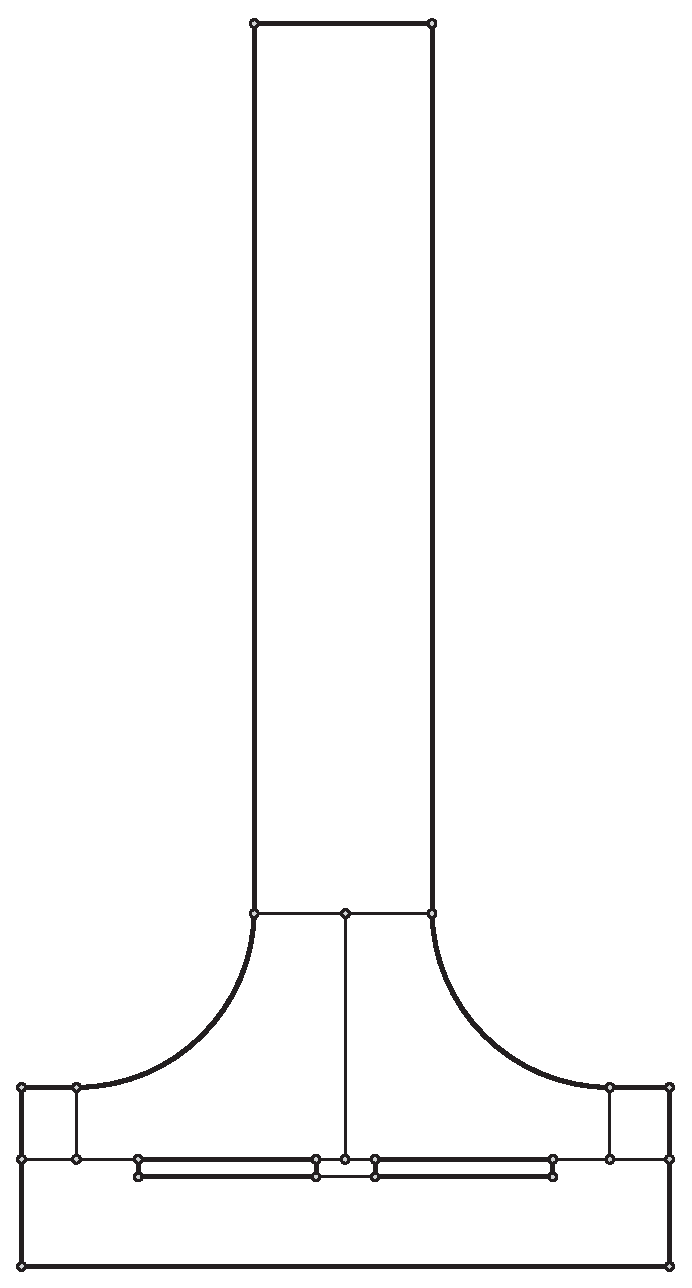
\includegraphics[width=.7\linewidth]{fig/divisionPelton1.eps}
		\caption{Mallable con triángulos solamente.}
	\end{subfigure}
	\begin{subfigure}{0.49\textwidth}
		\centering
		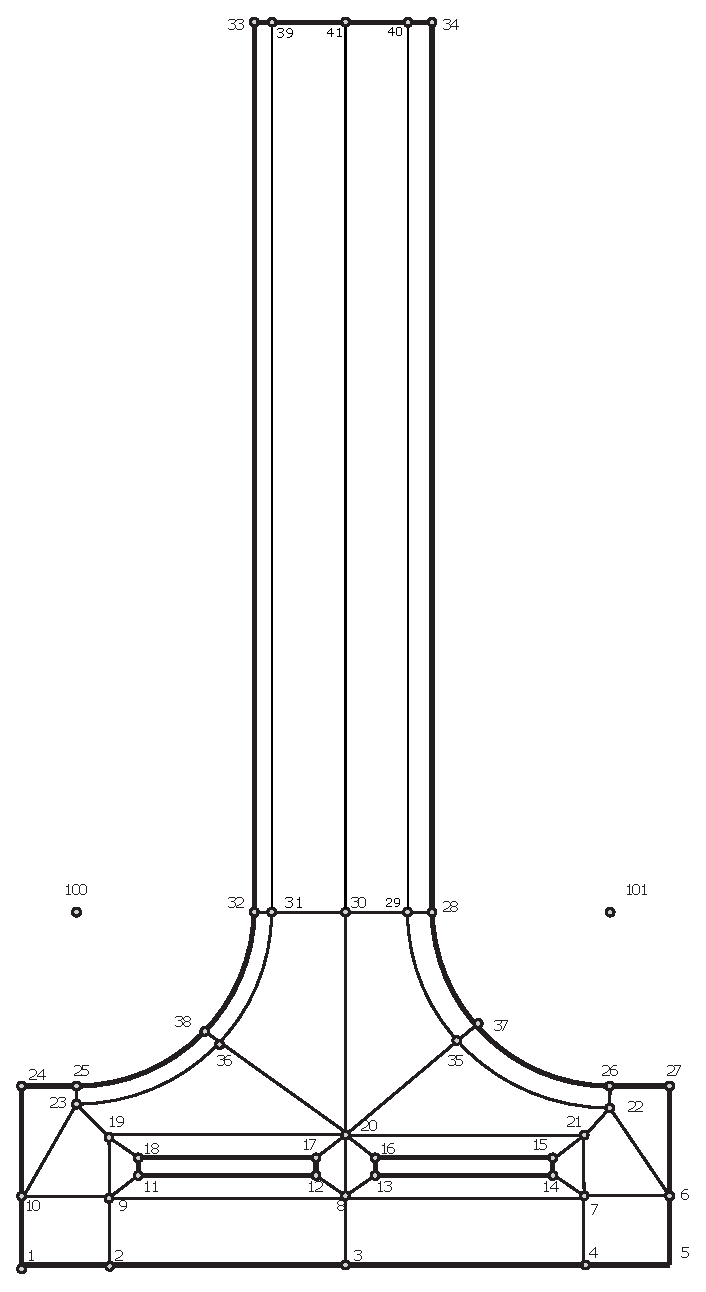
\includegraphics[width=.7\linewidth]{fig/divisionPelton2.eps}
		\caption{Se puede mallar con elementos cuadrilateros. No hay esquinas angulosas. Es posible obtener \textit{una buena malla}. Los puntos 100 y 101 son auxiliares y no forman parte de la malla.}
		\label{fig:buendivisiondominio}
	\end{subfigure}
	\caption{Dos formas de dividir una paleta de una turbina pelton que recibe un chorro incidente en su esquina superior derecha.}
\end{figure}
\begin{figure}[htb!]
	\centering
	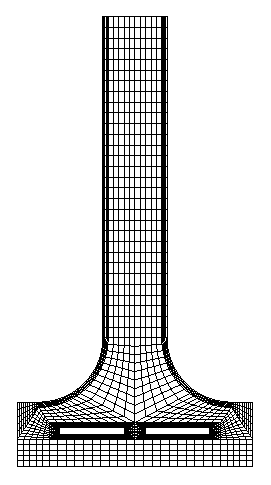
\includegraphics[angle=90,width=\linewidth]{fig/mallaPelton.eps}
	\caption{Ejemplo de malla usando divisiones de  \ref{fig:buendivisiondominio}. Se refina en los costados donde se tiene flexión.}
\end{figure}

%\clearpage
Protip: Necesitas saber que fuerza se tiene que hacer para que se mantenga en posición una arista o punto dado cargas térmicas/fuerza? Apoyalo (fix) y mira las reacciones con la carga térmica/fuerza.






\section{Funciones de formas para elementos 2D}
Las funciones de forma caracterizan un campo sobre un elemento y permiten interpolar valores dentro de este mismo. Esto nos permite integrar campos sobre ele elemento para la resolución del problema de elementos finitos. 

\subsection*{Cálculo}
Para calcular las funciones de forma primero se define cuantos nodos se va tener por elemento y se los ubica en el espacio $(x,y)$. Con el triangulo de Pascal para polinomios se elige el grado del polinomio y los términos. Luego se resuelve el sistema de ecuaciones $\MN\cdot X= A$ donde $\MN=[N_1\ms N_2 \ms \ldots\ms N_n]$ y $X=[1\ms x\ms y \ms\ldots\ms x^{k-1}y^{k} \ms x^{k}y^{k}]^T$, o algo por el estilo. Se tienen que elegir los grados mas convenientes teniendo en cuenta la simetría y el número de nodos, este ultimo te limita el número de términos posibles por la naturaleza de la interpolación. La matriz $A$ tendrá en su \textbf{espacio fila} el mismo polinomio evaluado en la posición del nodo correspondiente a esa fila.

\[
A=
\begin{bmatrix}
1 & x_1 & y_1 & \dots  & x_{1}^{k-1}y_1^{k} & x_{1}^{k}y_1^{k} \\
1 & x_2 & y_2 & \dots  & x_{2}^{k-1}y_2^{k} & x_{2}^{k}y_2^{k} \\
\vdots & \vdots & \vdots & \ddots & \vdots& \vdots \\
1 & x_n & y_n & \dots  & x_{n}^{k-1}y_n^{k} & x_{n}^{k}y_n^{k}
\end{bmatrix}
\]
Luego, las funciones de forma $\MN$ se pueden obtener así: $\MN=X^{-1} A$

Se habla de interpolación de campo en la sección de elementos isoparamétricos.

\section*{Cargas 2-D}
La ecuación que rige como se cargan elementos, siendo $\Cme{r}$ las cargas nodales del elemento, $\Cme{F}$ fuerzas volumétricas, $\CPhi$ fuerzas de tracción superficiales, $\Cme{\varepsilonb_0}$ las deformaciones iniciales y $\Cme{\sigmab_0}$ las tensiones iniciales (pg. 228)
\begin{equation} \label{eq:CargasGenerales}
\Cme{r}=\overbrace{\int \MN^T \Cme{F} \di V}^{\text{Volumétricas}} + \overbrace{\int \MN^T \CPhi \di S}^{\text{Superficiales}}+\int \MB^T \ME \Cme{\varepsilonb_0} \di V- \int \MB \Cme{\sigmab_0} \di V
\end{equation}



\section{Elementos isoparamétricos}
La formulación isoparamétrica permite interpolar campos sobre elementos cuadriláteros no rectangulares usando las mismas funciones de forma.

Se utiliza un sistema de coordenadas auxiliar $(\xi,\eta)$ en dos dimensiones y $(\xi,\eta,\zeta)$ en tres dimensiones. Para integrar se utiliza un método numérico llamado \textit{Cuadratura de Gauss}.



\begin{figure}
	\centering
	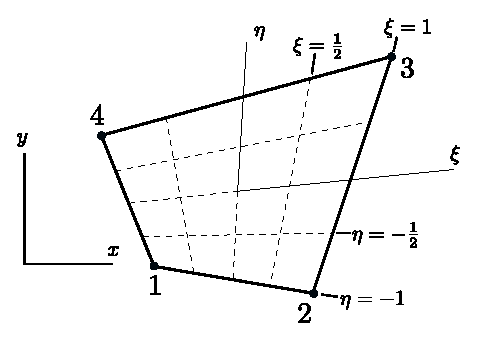
\includegraphics[width=8cm]{fig/q4isoparam.eps}
	\caption{Elemento Q4 en el espacio físico $(x,y)$. Sistema de referencia auxiliar $(\xi,\eta)$ visible. 
		%No necesariamente tienen que ser paralelas a $(x,y)$ ni ortogonales entre sí.
	}
	\label{fig:q4isoparam}
\end{figure}

\begin{itemize}
	\item Un elemento que no esta distorsionado (sigue siendo un rectangulo o paralelogramo) tiene $\jac$ constante
	\item Cuidado con modo espurio. Ver tabla 6.8-1 pg. 226 el tema de full/reduced integration \cite{cook2007concepts}
	\item Como cargar tu elemento isoparamétrico en pg. 228
\end{itemize}


\subsection*{Interpolación de campo}

Para interpolar el campo de interés (desplazamientos, coordenadas, tensión, etc.) es necesario conocer lo que vale el campo en los nodos del elemento.

Para interpolar el valor desconocido del campo $\phi$ sobre el punto $(x_d,y_d)$ se suma el producto de la función de forma evaluada en $(x_d,y_d)$ multiplicada por el campo en el nodo correspondiente
\[
\phi(x_d,y_d) = \sum_i^{\Nnodporelem} N_i(x_d,y_d) \cdot \phi(x_i,y_i) 
\]
Por ende, si se interpola sobre un nodo se debería obtener el valor del campo en el mismo nodo.


\subsection*{Integración usando cuadratura}
Para integrar un campo dentro de un elemento isoparamétrico se emplea el método de la cuadratura de Gauss. Se precisa integrar para obtener la matriz de rigidez de un sistema, las tensiones a partir de los desplazamientos y para obtener las cargas.

Para integrar se necesita conocer cuanto vale el campo sobre los denominados \textit{puntos Gauss} y multiplicar el valor por los pesos $W$ asociados al punto Gauss. Se suman estos valores para obtener la aproximación de la integral.
\begin{equation}
I=\int^1_{-1} \int^1_{-1}\phi(\xi,\eta) \di \xi \di \eta\approx \sum_i \sum_j W_i W_j \cdot \phi_{ij}(\xi,\eta) \cdot \Djac
\end{equation}
donde $\Djac$ es el determinante del jacobiano evaluado en el punto Gauss. Los pesos y las posiciones de los puntos Gauss se pueden calcular usando la función \texttt{gauss.m} del anexo (código \ref{cod:gauss}).

La matriz jacobiana, o simplemente \textit{jacobiano}, es un factor de escala que relaciona el incremento de longitud por la transformación $(\xi,\eta)\rightarrow(x,y)$. Para la transformación de coordenadas Cartesianas a polares $\di x~ \di y = r \cdot \di r~  \di \theta$ el determinante es $\Djac=r$.

\[
\jac = \begin{bmatrix}
\spartial{x}{\xi} & \spartial{y}{\xi} \\
\spartial{x}{\eta} & \spartial{y}{\eta}
\end{bmatrix}
\]

\begin{figure}[htb!]
	\centering
	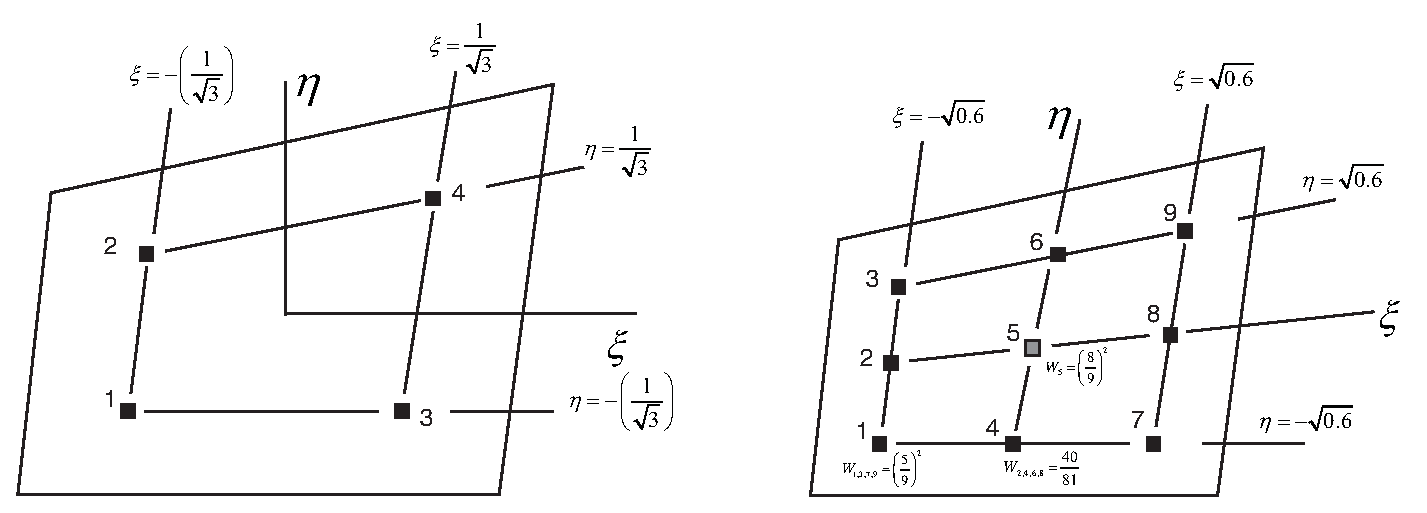
\includegraphics[width=12cm]{fig/gauss_n3.eps}
	\caption{Puntos Gauss para reglas $2\times 2$ y $3\times3$. El peso vale 1 en todos los puntos Gauss para la regla $2\times2$.}
	\label{fig:gauss_n3}
\end{figure}



\section*{Ejemplo elemento exótico}
\subsection*{Matriz de Rigidez}
Imaginemos un elementos Q5 (figura \ref{fig:elemq5}) cuadrado de dimensiones $2\times2$ con espesor $t$  (igual al Q4 con un nodo en su centro). Si fuéramos a obtener las funciones de formas de dicho elemento quedarían iguales para $(x,y)$ y para $(\xi,\eta)$ por las dimensiones usadas. La funcionalidad que uno estaría tentado a seleccionar sería $[1,\ x, \ y,\ x^2, \ y^2 ]$, pero está trae problemas inesperados debido a que tiene varias soluciones en la interpolación. Como nuestra prioridad siempre es mantener la simetría la funcionalidad será $[1,\ x,\ y,\ xy,\ x^2y^2 ]$.  Tomando el orden de la figura \ref{fig:elemq5}:
\[
\MN=\left[\begin{array}{ccccc} \frac{x^2\,y^2}{4}+\frac{x\,y}{4}-\frac{x}{4}-\frac{y}{4}, & \frac{x^2\,y^2}{4}-\frac{x\,y}{4}+\frac{x}{4}-\frac{y}{4}, & \frac{x^2\,y^2}{4}+\frac{x\,y}{4}+\frac{x}{4}+\frac{y}{4}, & \frac{x^2\,y^2}{4}-\frac{x\,y}{4}-\frac{x}{4}+\frac{y}{4}, & 1-x^2\,y^2 \end{array}\right]
\]

Llegado a este punto nos interesa obtener la matriz de rigidez. Si queremos lograr \emph{``full integration"} deberíamos usar Gauss orden $n=3$ según \eqref{eq:gaussinequality}

\begin{equation} \label{eq:gaussinequality}
2n-1\geq O\left(\MB^T \ME \MB \right)
\end{equation}


$\MB$ es el \textit{strain-deformation matrix}. El producto $\MB^T \ME \MB$ da un polinomio de orden 6 ($\MB$ tiene el mismo orden que la derivada de $\MN$). De esta forma nos aseguramos que nuestro resultado va ser exacto para el elemento sin distorsionar.

Para esté ejemplo, no se pide \emph{full integration} entonces no pasa nada si queremos \emph{underintegrate}. Usamos Gauss orden $n=2$. 

\begin{figure}[htb!]
	\centering
	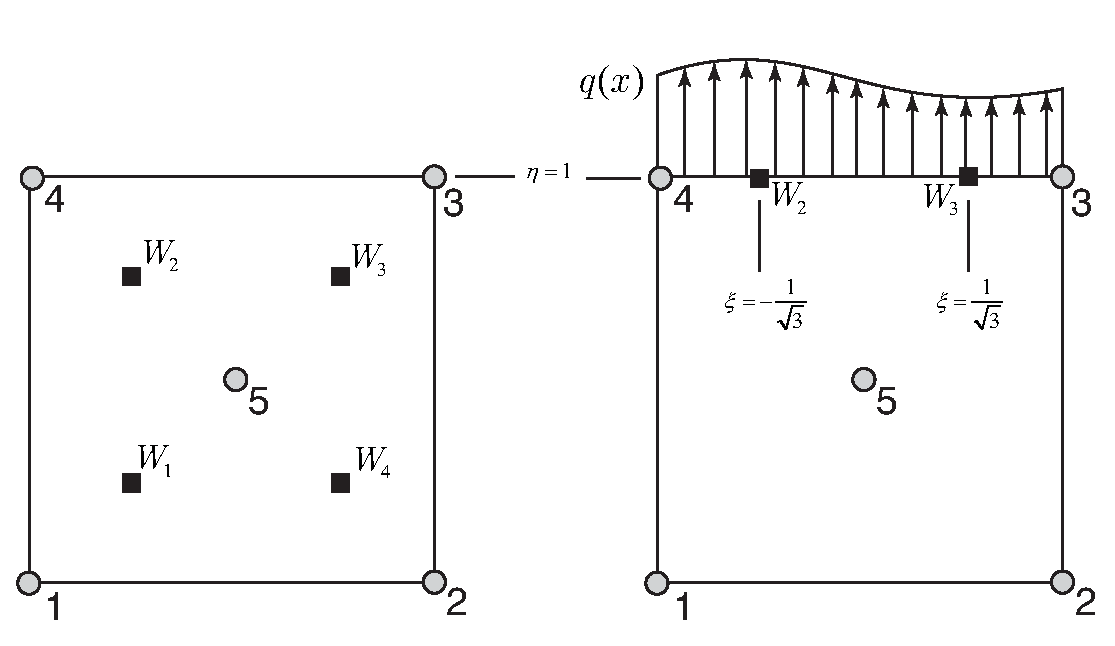
\includegraphics[height=5cm]{fig/exoticElement.eps}
	\caption{Elemento Q5 rectangular.}
	\label{fig:elemq5}
\end{figure}

La rigidez de un elemento está dada por 


\begin{equation} \label{eq:RigidezElemento}
\Mk=\int \MB^T \ME \MB \di V
\end{equation}
para un elemento plano la ecuación anterior es
\[
\Mk_{\mathrm{2D}}=\iint \MB^T \ME \MB t \di x \di y=\int^1_{-1}\int^1_{-1} \MB^T \ME \MB t \ \Djac \  \di\xi  \di\eta
\]
donde $\MB$ es la matriz deformación-desplazamiento del elemento, $\ME$ es la matriz constitutiva, y $\Djac$ es el determinante de la matriz Jacobiana, el cual se le suele decir simplemente el Jacobiano.

Este ultimo se calcula a partir de la derivada de las funciones de forma $ $

\subsection*{Carga de linea}
Si el elemento está cargado sobre la linea 4-3 con una distribuida $q(x)$ (en [N/m]) entonces procedemos de la siguiente manera según el segundo término de \refp{eq:CargasGenerales}: 

\begin{align}
r_{xi}&=\int^1_{-1}N_i (\tau \jac_{11}- \sigma \jac_{12})t\di \xi \\
r_{yi}&=\int^1_{-1}N_i (\sigma \jac_{11}+\tau \jac_{12})t \di \xi 
\end{align}
donde $\sigma$ es la solicitación normal a la superficie y $\tau$ es la tangencial. Para la fuerza sobre el nodo 4 se tiene

$$r_{y4}= N_4(\xi_2)t\left[\sigma(\xi_2)\; \jac_{11}+\tau(\xi_2)\; \jac_{12}\right] \cdot W_2 + N_4(\xi_3)t\left[\sigma(\xi_3)\; \jac_{11}+\tau(\xi_3)\; \jac_{12}\right]\cdot W_3 $$

Si consideramos que solo hay una \emph{carga distribuida de linea} a tracción/compresión como indica la figura \ref{fig:elemq5}, se reduce la ecuación anterior

$$ r_{y4} = N_4(\xi_2)\;\jac_{11}\;q(\xi_2) + N_4(\xi_3)\;\jac_{11}\;q(\xi_3) =N_4\;q \;\jac_{11}\Big|_{\xi_2} + N_4\;q\; \jac_{11}\Big|_{\xi_3} $$
similarmente $r_{y3} = N_3\;q \;\jac_{11}\big|_{\xi_2} + N_3\;q\; \jac_{11}\big|_{\xi_3} $ donde la matriz Jacobiana también se evalúa para cada punto de Gauss!


\subsection*{Tensiones}
\begin{itemize}
	\item Las tensiones en los nodos suele ser de mayor interés que sobre los puntos de gauss (mas comprometidas, permiten estimar error)
\end{itemize}

\section{Elementos Axisimetricos}
Resuelvo problema 3-D en el plano. \textbf{Los resultados son por cada unidad radian}. Como sigo teniendo dos grados de libertad tengo las mismas funciones de forma. Cambia mi operador derivada.
\[
\begin{Bmatrix}
\sigma_\radial \\
\sigma_\theta \\
\sigma_z \\
\tau_{z\radial}
\end{Bmatrix}
= \frac{(1-\nu)E}{(1+\nu)(1-2\nu)}
\begin{bmatrix}
1 & \eff & \eff & 0 \\
& 1 & \eff & 0 \\
& & 1 & 0 \\
\textrm{sim.}\unspace& & & g 
\end{bmatrix}
\left(
\begin{Bmatrix}
\varepsilon_\radial \\
\varepsilon_\theta \\
\varepsilon_z \\
\gamma_{\radial z}
\end{Bmatrix}
-
\begin{Bmatrix}
\alpha T\\
\alpha T \\
\alpha T \\
0
\end{Bmatrix}
\right)
\]
donde 
\[
f=\frac{\nu}{1-\nu}\qquad \quad \textrm{y}\quad \qquad g=\frac{1-2\nu}{2(1-\nu)}
\]

Una carga puntual $P$ aplicada sobre un elemento axisimétrico no tiene el mismo significado físico que en elementos plane stress/strain. 
\[
P=2\pi rq
\]
donde $q$ es la carga distribuida en [N/m], $r$ es la distancia al eje de revolución y $2 \pi$ es el resultado de integrar la fuerza distribuida sobre $\theta$. 

\[
\Cme{r_e} = \int\int_{-\pi}^{\pi} \MN^T \begin{Bmatrix}
\rho r \omega ^2 \\
0
\end{Bmatrix} r \di \theta \di A
\]